\chapter{KẾT LUẬN VÀ HƯỚNG PHÁT TRIỂN}
\label{conclusion}
\paragraph{Chương 5} sẽ trình bày kết quả của quá trình huấn luyện dữ liệu mà nhóm chuẩn bị với mô hình Faster R-CNN đồng thời tự đánh giá về những việc đã và chưa làm được của nhóm, từ đó đưa ra hướng phát triển cho đề tài.

\section{Kết quả}
Dựa trên kết quả thu được từ 2 tập dữ liệu đánh giá, ta có cái nhìn tổng quát về quá trình và kết quả huấn luyện như sau:
\begin{itemize}
	\item Đối với hình ảnh có những trái to, rõ ràng, mô hình mạng đã nhận diện được chính xác và khá đầy đủ
	\item Đối với những hình ảnh cây có quá nhiều lá, lá che phần lớn các trái, mô hình mạng nhận diện được đúng các trái, tuy nhiên vẫn còn nhận dư và nhận thiếu các trái
	\item Cần cải thiện đối với những trường hợp trái bị che bởi cành, lá dẫn đến không nhận diện được, đưa tới kết quả là thiếu trái, được thể hiện bởi False Negative
	\item Các trường hợp nhận nhầm các vùng cành lá thành trái (False Positive) cũng rất đáng được quan tâm và cải thiện
\end{itemize}
Để giải quyết hai vấn đề trên, nhóm đã đề xuất hướng giải quyết là đưa những vùng nhận diện được là trái bưởi qua các một CNN để phân loại.
Nhóm đã chuẩn bị tập dữ liệu với 14496 hình dùng cho việc huấn luyện và 7248 hình dùng cho việc kiểm tra, với hai class là có trái và không trái.
\begin{center}
    \begin{figure}[H]
    \centering
    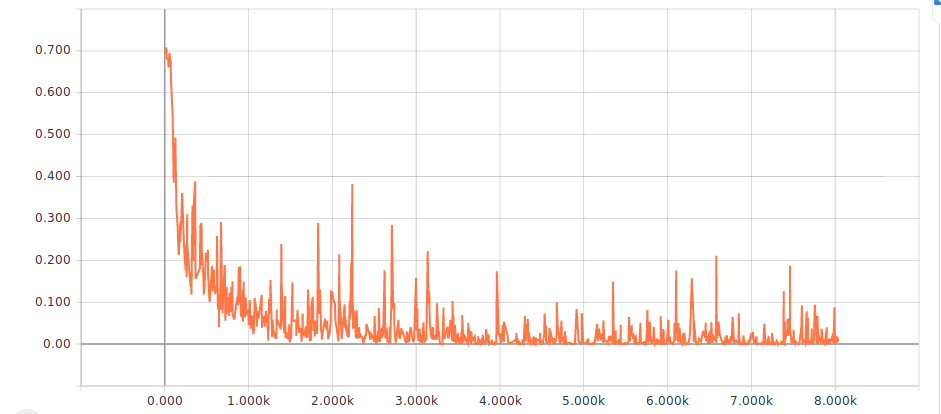
\includegraphics[width=0.7\columnwidth]{images/chap3/loss_cls_full.png}
    \caption{Biểu đồ lỗi khi huấn luyện CNN phân loại ảnh có trái bưởi}
    \label{fig:my_label}
    \end{figure}
\end{center}
Kết quả huấn luyện cho độ chính xác 0.991 đối với tập dữ liệu kiểm tra, tuy nhiên khi áp dụng vào bộ phân loại vẫn chưa cho được hiệu quả như nhóm mong muốn, việc phân loại sai còn khá nhiều.\\
Từ kết quả thực nghiệm, có thể thấy được rằng việc áp dụng mô hình Faster R-CNN cho bài toán nhận diện và đánh giá năng suất cây ăn trái ở Việt Nam là khả thi, tuy nhiên cần áp dụng thêm nhiều biện pháp trong quá trình tiền xử lí và huấn luyện, đồng thời cần lượng dữ liệu lớn hơn để giúp mô hình hoạt động hoàn hảo hơn.
\section{Kết luận}
\subsection{Những việc đã làm được}
\begin{itemize}
\item Tìm hiểu các tổng quát lí thuyết và các phương pháp áp dụng thị giác máy tính và xử lí ảnh để giải quyết bài toán và những nghiên cứu liên quan

\item Tìm hiểu về mô hình mạng nơ-ron nhân tạo ANN, lí thuyết, kiến trúc và cách hoạt động của nó

\item Tìm hiểu về mô hình mạng CNN, cấu tạo của các lớp convolutional, lớp pooling và các hàm kích hoạt thường được sử dụng để giải quyết bài toán với dữ liệu hình ảnh

\item Tìm hiểu và thực hiện quá trình lấy mẫu ảnh cho ảnh thực tế, tiền xử lý ảnh, , augmentation để đa dạng hóa tập ảnh gốc, nhằm giúp nâng cao độ chính xác cho mô hình mạng

\item Tiến hành tìm hiểu thư viện Tensorflow, chỉnh sửa mã nguồn để áp dụng vào bài toán nhận diện trái bưởi

\item Tiến hành các quá trình huấn luyện, chỉnh sửa lỗi phát sinh của mã nguồn

\item Tìm hiểu và thực hiện các công đoạn đánh giá kết quả huấn luyện, chọn những mô hình cho kết quả tốt nhất, từ đó xem xét tính khả thi để áp dụng vào thực tiễn

\item Xây dựng được mô hình nhận diện trái bưởi ở nước ta với độ chính xác khá cao

\end{itemize}

\subsection{Những việc chưa làm được}
\begin{itemize}
\item Mô hình nhận diện vẫn còn các vùng bị sai và bị thiếu trái đặc biệt là ở những vùng bị lá che
\item Tập dữ liệu nhóm xây dựng còn khá nhỏ, do việc thu thậm dữ liệu thực tế khá khó khăn
\item Chưa xây dựng được ứng dụng để áp dụng giải thuật trên các thiết bị di động
\end{itemize}

\section{Hướng phát triển}
Đề tài này có nhiều hướng phát triển trong tương lai như:
\begin{itemize}
\item Tìm hiểu thêm các phương pháp để xử lí những vùng bị lá che để tăng thêm độ chính xác cho mô hình
\item Xây dựng tập dữ liệu lớn hơn, và mở rộng ra nhiều loại trái cây hơn
\item Tìm hiểu quy trình, phương pháp xây dưng và hiện thực ứng dụng để có thể sử dụng rộng rãi
\end{itemize}
